% This file was created with matplot2tikz v0.5.1.
% This file was created with matplot2tikz v0.5.1.
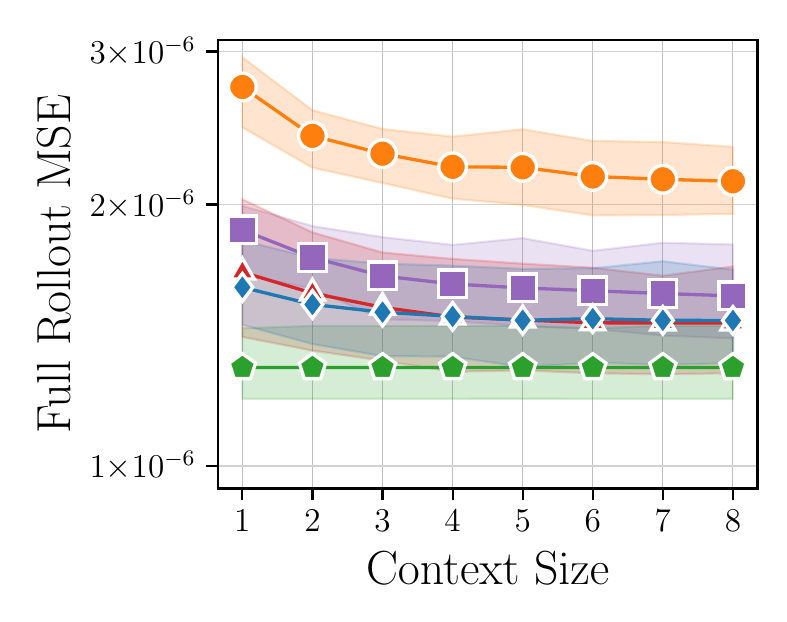
\begin{tikzpicture}
\definecolor{crimson2143940}{RGB}{214,39,40}
\definecolor{darkgray}{RGB}{169,169,169}
\definecolor{darkorange25512714}{RGB}{255,127,14}
\definecolor{darkslategray38}{RGB}{38,38,38}
\definecolor{forestgreen4416044}{RGB}{44,160,44}
\definecolor{lightgray204}{RGB}{204,204,204}
\definecolor{mediumpurple148103189}{RGB}{148,103,189}
\definecolor{steelblue31119180}{RGB}{31,119,180}

\begin{axis}[
    line width=0.8pt, % Makes the axis outline thicker/darker
    axis line style={black}, % Use solid black for maximum contrast
    log basis y={10},
    % Combined minor and major ticks
    ytick={1e-06, 2e-06, 3e-06, 4e-06, 6e-06, 1e-05, 2e-05, 3e-05, 4e-05, 6e-05, 1e-04, 2e-04, 3e-04, 4e-04, 6e-04},
    yticklabels={
        \(1{\times}10^{-6}\), \(2{\times}10^{-6}\), \(3{\times}10^{-6}\), \(4{\times}10^{-6}\), \(6{\times}10^{-6}\),
        \(10^{-5}\), \(2{\times}10^{-5}\), \(3{\times}10^{-5}\), \(4{\times}10^{-5}\), \(6{\times}10^{-5}\),
        \(10^{-4}\), \(2{\times}10^{-4}\), \(3{\times}10^{-4}\), \(4{\times}10^{-4}\), \(6{\times}10^{-4}\)
    },
    tick align=outside,
    % title={Deforming Block},
    xlabel={Context Size},
    xlabel style={font=\LARGE, color=black},
    ylabel={Full Rollout MSE}, % Added ylabel back
    ylabel style={font=\LARGE, color=black}, % Matching the "Darker" style
    tick label style={font=\large, color=black}, % Matching the "Darker" style
    xmajorgrids,
    xtick={1,2,3,4,5,6,7,8},           % Specify tick positions
    xticklabels={1,2,3,4,5,6,7,8},     % Specify tick labels
    xmajorticks=true,                  % Ensure ticks are enabled
    xtick pos=bottom,
    xmin=0.65, xmax=8.35,
    xtick style={color=black, line width=0.8pt},
    y grid style={lightgray!70}, % Slightly darker grid for better visibility
    ymajorgrids,
    ymin=0.94208220010013e-06, ymax=3.09143132540889e-06,
    ymode=log,
    ytick pos=left,
    ytick style={color=black, line width=0.8pt}
]
\path [draw=darkorange25512714, fill=darkorange25512714, opacity=0.2]
(axis cs:1,2.95462405119906e-06)
--(axis cs:1,2.45336601238932e-06)
--(axis cs:2,2.20497292957589e-06)
--(axis cs:3,2.11740757549705e-06)
--(axis cs:4,2.03107032348271e-06)
--(axis cs:5,1.9985720882687e-06)
--(axis cs:6,1.94296484323786e-06)
--(axis cs:7,1.94556162114168e-06)
--(axis cs:8,1.95145361203686e-06)
--(axis cs:8,2.32996734439439e-06)
--(axis cs:8,2.32996734439439e-06)
--(axis cs:7,2.3596542746418e-06)
--(axis cs:6,2.36665329111929e-06)
--(axis cs:5,2.44106007585287e-06)
--(axis cs:4,2.39378744595342e-06)
--(axis cs:3,2.4429660925307e-06)
--(axis cs:2,2.56724428027155e-06)
--(axis cs:1,2.95462405119906e-06)
--cycle;
\path [draw=mediumpurple148103189, fill=mediumpurple148103189, opacity=0.2]
(axis cs:1,1.99352103891215e-06)
--(axis cs:1,1.66243012245104e-06)
--(axis cs:2,1.59966228352459e-06)
--(axis cs:3,1.47524616522787e-06)
--(axis cs:4,1.46801022538057e-06)
--(axis cs:5,1.44900729992514e-06)
--(axis cs:6,1.43809398878147e-06)
--(axis cs:7,1.41286835741994e-06)
--(axis cs:8,1.40251364655342e-06)
--(axis cs:8,1.79910261977057e-06)
--(axis cs:8,1.79910261977057e-06)
--(axis cs:7,1.80700888563479e-06)
--(axis cs:6,1.76912186589107e-06)
--(axis cs:5,1.82960323513726e-06)
--(axis cs:4,1.79694262669727e-06)
--(axis cs:3,1.8341795851029e-06)
--(axis cs:2,1.88873465845063e-06)
--(axis cs:1,1.99352103891215e-06)
--cycle;
\path [draw=crimson2143940, fill=crimson2143940, opacity=0.2]
(axis cs:1,2.02769706447725e-06)
--(axis cs:1,1.40788753810739e-06)
--(axis cs:2,1.35791756861181e-06)
--(axis cs:3,1.32207259184725e-06)
--(axis cs:4,1.2835851350701e-06)
--(axis cs:5,1.28860116888063e-06)
--(axis cs:6,1.27854914921954e-06)
--(axis cs:7,1.27543921735196e-06)
--(axis cs:8,1.27874079680623e-06)
--(axis cs:8,1.69665094063021e-06)
--(axis cs:8,1.69665094063021e-06)
--(axis cs:7,1.65599628800805e-06)
--(axis cs:6,1.69140358252662e-06)
--(axis cs:5,1.70982760820948e-06)
--(axis cs:4,1.73124954017112e-06)
--(axis cs:3,1.76100652993227e-06)
--(axis cs:2,1.85751306958082e-06)
--(axis cs:1,2.02769706447725e-06)
--cycle;
\path [draw=forestgreen4416044, fill=forestgreen4416044, opacity=0.2]
(axis cs:1,1.44048956940424e-06)
--(axis cs:1,1.1951971146118e-06)
--(axis cs:2,1.19520160524189e-06)
--(axis cs:3,1.19519444297111e-06)
--(axis cs:4,1.19517227403776e-06)
--(axis cs:5,1.19496376811412e-06)
--(axis cs:6,1.19520450425625e-06)
--(axis cs:7,1.19520740327062e-06)
--(axis cs:8,1.19519626196052e-06)
--(axis cs:8,1.4497597362606e-06)
--(axis cs:8,1.4497597362606e-06)
--(axis cs:7,1.44975774674094e-06)
--(axis cs:6,1.44050022754527e-06)
--(axis cs:5,1.44975012972282e-06)
--(axis cs:4,1.44973930105152e-06)
--(axis cs:3,1.44975649618573e-06)
--(axis cs:2,1.44974879390247e-06)
--(axis cs:1,1.44048956940424e-06)
--cycle;
\path [draw=steelblue31119180, fill=steelblue31119180, opacity=0.2]
(axis cs:1,1.81762419515508e-06)
--(axis cs:1,1.45395972594997e-06)
--(axis cs:2,1.38173538744013e-06)
--(axis cs:3,1.33824292376517e-06)
--(axis cs:4,1.33626258502773e-06)
--(axis cs:5,1.29966741724274e-06)
--(axis cs:6,1.31520494051074e-06)
--(axis cs:7,1.30778784068752e-06)
--(axis cs:8,1.31355028543112e-06)
--(axis cs:8,1.68259728638986e-06)
--(axis cs:8,1.68259728638986e-06)
--(axis cs:7,1.72052705238457e-06)
--(axis cs:6,1.68917330256591e-06)
--(axis cs:5,1.6862453549038e-06)
--(axis cs:4,1.70081307260261e-06)
--(axis cs:3,1.70971210877724e-06)
--(axis cs:2,1.73661598523722e-06)
--(axis cs:1,1.81762419515508e-06)
--cycle;
\addplot [very thick, darkorange25512714, mark=*, mark size=5, mark options={solid,draw=white}]
table {%
1 2.73071873380104e-06
2 2.39898594145416e-06
3 2.28819567382743e-06
4 2.2100099954514e-06
5 2.20702219166924e-06
6 2.15425234273425e-06
7 2.13807220461604e-06
8 2.1268699583743e-06
};
\addplot [very thick, mediumpurple148103189, mark=square*, mark size=5, mark options={solid,draw=white}]
table {%
1 1.87011249863644e-06
2 1.73767040223538e-06
3 1.65489782943951e-06
4 1.62000515047112e-06
5 1.60325535603079e-06
6 1.59140887490139e-06
7 1.57951745904938e-06
8 1.56983574584046e-06
};
\addplot [very thick, crimson2143940, mark=triangle*, mark size=5, mark options={solid,draw=white}]
table {%
1 1.67174763987532e-06
2 1.58122753646239e-06
3 1.52279605458716e-06
4 1.48431567481566e-06
5 1.4726347501437e-06
6 1.46166718195673e-06
7 1.4611167671319e-06
8 1.4608461356147e-06
};
\addplot [very thick, forestgreen4416044, mark=pentagon*, mark size=5, mark options={solid,draw=white}]
table {%
1 1.29855533259615e-06
2 1.29855405361923e-06
3 1.29855956743086e-06
4 1.29854697661358e-06
5 1.29855263253376e-06
6 1.29855817476709e-06
7 1.29856246644522e-06
8 1.29856201169787e-06
};
\addplot [very thick, steelblue31119180, mark=diamond*, mark size=5, mark options={solid,draw=white}]
table {%
1 1.60576516350375e-06
2 1.5344699590969e-06
3 1.50345218230541e-06
4 1.48669604982388e-06
5 1.47146081985738e-06
6 1.47769040381718e-06
7 1.47124487170913e-06
8 1.47071213518757e-06
};
\end{axis}
\end{tikzpicture}